\documentclass[
12pt,
 a4paper,
 % chapter=TITLE,
  % section=TITLE,
   % subsection=TITLE,
    % subsubsection=TITLE,
    english,
    brazil,
    % openright,
    % twoside
    oneside
    ]{abntex2}
    
% Pacotes
% ---
\usepackage[brazilian,hyperpageref]{backref}
\usepackage[alf]{abntex2cite}
\usepackage[utf8]{inputenc}
\usepackage[T1]{fontenc}
\usepackage{amsmath, amsfonts, amssymb}
\usepackage{float}
\usepackage{graphicx}
\usepackage{indentfirst}
\usepackage{hyperref}
\usepackage{geometry}
\usepackage{times}
\usepackage{setspace}
\usepackage{microtype}
\usepackage{color}
\usepackage{tikz} 
\usetikzlibrary{positioning,shapes.geometric}
% ---


% Configurações de margens
\geometry{
	a4paper,
	left=3cm,
	right=2cm,
	top=3cm,
	bottom=2cm
}

% Configurações do pacote backref
% Usado sem a opção hyperpageref de backref
\renewcommand{\backrefpagesname}{Citado na(s) página(s):~}
% Texto padrão antes do número das páginas
\renewcommand{\backref}{}
% Define os textos da citação
\renewcommand*{\backrefalt}[4]{
	\ifcase #1 %
	%
	\or
	Citado na página #2.%
	\else
	Citado #1 vezes nas páginas #2.%
	\fi}%
% ---

% Dados do TCC/Monografia
\titulo{Transformações Lineares e suas aplicações}
\autor{Hyslan Silva Cruz\\Iara Regina Grilo Papais\\Carolina Cristina Ferreira de Mello Pires}
\orientador[Orientadora:]{Lorena Salvi Stringheta}
\instituicao{Universidade Virtual do Estado de São Paulo} 
\local{Suzano}
\data{2024}
\tipotrabalho{TCC}
\preambulo{Monografia de graduação à Universidade Virtual do Estado de São Paulo, como requisito parcial para a obtenção do título de Licenciatura em Matemática.
	\\Orientadora: \imprimirorientador}


% Configurações de aparência do PDF final
% alterando o aspecto da cor azul
\definecolor{blue}{RGB}{41,5,195}

% informações do PDF
\makeatletter
\hypersetup{
	%pagebackref=true,
	pdftitle={\@title}, 
	pdfauthor={\@author},
	pdfsubject={\imprimirpreambulo},
	pdfcreator={LaTeX with abnTeX2},
	pdfkeywords={abnt}{latex}{abntex}{abntex2}{trabalho acadêmico}, 
	colorlinks=true,       		% false: boxed links; true: colored links
	linkcolor=black,          	% color of internal links
	citecolor=black,        		% color of links to bibliography
	filecolor=magenta,      		% color of file links
	urlcolor=blue,
	bookmarksdepth=4
}
\makeatother
% --- 

% ---
% Posiciona figuras e tabelas no topo da página quando adicionadas sozinhas
% em um página em branco. Ver https://github.com/abntex/abntex2/issues/170
\makeatletter
\setlength{\@fptop}{5pt} % Set distance from top of page to first float
\makeatother
% ---

% --- 
% Espaçamentos entre linhas e parágrafos 
% --- 

% O tamanho do parágrafo é dado por:
\setlength{\parindent}{1.3cm}

% Controle do espaçamento entre um parágrafo e outro:
\setlength{\parskip}{0.2cm}  % tente também \onelineskip

% Início do Documento
\begin{document}
	
	\selectlanguage{brazil}
	
	% Retira espaço extra obsoleto entre as frases.
	\frenchspacing 
	
	
	\renewcommand{\imprimircapa}{%
		\begin{capa}%
			\center
			{\ABNTEXchapterfont\large\imprimirautor}
			\vspace*{\fill}
			
			{\ABNTEXchapterfont\bfseries\LARGE\imprimirtitulo}
			
			\vspace*{5cm}
			\href{teste.com.br}{\textbf{Link do vídeo}}
			\vspace*{\fill}
			
			{\large\imprimirlocal}
			\par
			{\large\imprimirdata}
			\vspace*{1cm}
		\end{capa}
	}
	% Capa
	\imprimircapa
	% \href{teste.com.br}{video}
	
	% Folha de Rosto
	\imprimirfolhaderosto
	
	% ---
	% Dedicatória
	% ---
	\begin{dedicatoria}
		\vspace*{\fill}
		\centering
		\noindent
		\textit{
			Este trabalho é dedicado às crianças adultas que,\\
			quando pequenas, sonharam em se tornar cientistas.\\
			}
	\end{dedicatoria}
	% ---
	
	% ---
	% Agradecimentos
	% ---
	\begin{agradecimentos}
		A conclusão desta monografia representa um marco importante em nossas vidas acadêmica e profissional. Ao longo dessa jornada, tivemos a oportunidade de contar com o apoio e a colaboração de diversas pessoas e instituições, às quais expresso minha mais profunda gratidão.
		
		À minha família e amigos,
		
		minha base sólida e porto seguro em todos os momentos. Agradeço por acreditarem em nosso potencial, por incentivarem nossos sonhos e por celebrarem cada conquista ao nosso lado. A vocês, dedico este trabalho com imenso amor e reconhecimento.
		
		A  minha orientadora, Professora \imprimirorientador,
		
		reconheço a importância fundamental de sua orientação, sabedoria e paciência ao longo da pesquisa. Sua expertise e dedicação nos inspiraram e guiaram na construção deste trabalho. Agradeço pelas valiosas contribuições, pelo tempo dedicado e pela confiança depositada em nosso grupo.
		
		Aos demais membros da banca examinadora,
		
		Professores(as),
		
		agradeço a oportunidade de apresentar nossa pesquisa e receber seus valiosos feedbacks. Agradeço por terem dedicado seu tempo e conhecimento à avaliação deste trabalho.
		
		À \imprimirinstituicao,
		
		minha segunda casa durante os anos de graduação. Agradeço à instituição por nos proporcionar uma formação de qualidade, por nos colocar em contato com professores excepcionais e por nos oferecer os recursos necessários para o desenvolvimento desta pesquisa de forma gratuita.
		
		Aos colegas de curso e amigos da Licenciatura em Matemática,
		
		com quem compartilhamos momentos de aprendizado, desafios e alegrias. Agradeço pelas trocas de conhecimento, pelo apoio mútuo e pela amizade que nos acompanham desde o início da graduação.
		
		Aos projetos integradores e demais serviços de pesquisa além da plataforma acadêmica,
		
		que nos proporcionaram acesso a materiais essenciais para a realização deste trabalho. Agradeço a todos os profissionais que me auxiliaram na busca por informações e na utilização de ferramentas para uma boa pesquisa.
		
		A todos que, direta ou indiretamente, contribuíram para a realização deste trabalho,
		
		nossa sincera gratidão. Cada palavra de incentivo, cada sugestão e cada ajuda foram valiosas para o nosso aprimoramento e para a conquista deste objetivo.
		
		Este trabalho é fruto de um esforço coletivo e representa a soma de conhecimentos, experiências e apoio de muitas pessoas. Agradecemos a todos que fizeram parte dessa jornada e que nos ajudaram a alcançar este importante marco em nossas vidas.
	\end{agradecimentos}
	% ---
	
	% ---
	% Epígrafe
	% ---
	\begin{epigrafe}
		\vspace*{\fill}
		\begin{flushright}
			\textit{``Hoje, ainda almejamos saber por que\\
				estamos aqui e de onde viemos.O desejo\\
				profundo da humanidade pelo	conhecimento é\\
				justificativa suficiente para nossa busca contínua.\\
				(Stephen Hawking)}
		\end{flushright}
	\end{epigrafe}
	% ---
	
	
	% Resumo
	% resumo em português
	\setlength{\absparsep}{18pt} % ajusta o espaçamento dos parágrafos do resumo
	\begin{resumo}
		Só após ao fim da conclusão.
		
		\textbf{Palavras-chave: Transformação Linear, Álgebra Linear, Matrizes}
	\end{resumo}
		
	
	% Abstract
	% resumo em inglês
	\begin{resumo}[Abstract]
		\begin{otherlanguage*}{english}
			Same above.
			
			\vspace{\onelineskip}
			
			\noindent 
			\textbf{Keywords}: Linear Transformation, Linear Algebra. Matrices.
		\end{otherlanguage*}
	\end{resumo}
	
	% inserir lista de tabelas
	% ---
	\pdfbookmark[0]{\listtablename}{lot}
	\listoftables*
	\cleardoublepage
	% ---
	
	% Lista de símbolos
	\begin{simbolos}
		\item[$ \mathbb{R} $] Conjunto dos números reais.
		\item[$\exists$] Existe.
		\item[$\in$] Pertence.
		\item[$\mid$] Tal que.
		\item[$\therefore$] Portanto.
		\item[$\emptyset$] Conjunto vazio.
		\item[$\sigma$] Somatório.
	\end{simbolos}
	
	
	% Sumário
	\pdfbookmark[0]{\contentsname}{toc}
	\tableofcontents*
	\cleardoublepage
	
	
	% Capítulos
	\textual
	
	\chapter{Introdução}
Com o decorrer do tempo, depois da era de ouro da álgebra linear nos meados de 1700. Não foi mais evidenciado como antigamente, para isto então, temas abordados nesse campo da matemática são frequentemente esquecidos
, para isto, este estudo trata de buscar o entendimento e compreender sobre as transformações lineares em sua totalidade.
		
	\chapter{Espaços Vetoriais}
Começaremos pela definição de um espaço vetorial utilizando aquelas apresentadas por \cite{boldrini1980} e \cite{ulhoa2018}, onde, podemos tratar como um vetor ao designar um elemento do espaço vetorial de um número $\mathbb{R}$ definido tal que:

\noindent\textbf{Definição 01:} Seja um conjunto V, não vazio, com duas operações: soma, $V \times V \rightarrow V$, e multiplicação por escalar, $R \times V \rightarrow V$, tais que, para quaisquer $u, v, w \in \mathbb{R}$, satisfaçam as propriedades: \nocite{boldrini1980}

\begin{enumerate}
	\item $(u + v) + w = u + (v + w), \forall$ $u, v, w \in V$ (propriedade associativa.) 
	\item $1u = u$.
	\item $u + v = v + u, \forall$ $u, v \in V$ (propriedade comutativa).
	\item $\exists$ $0$ $\in V$ tal que $u + 0 = u$.
	\item $\exists$ $-u \in V$ tal que $u + (-u) = 0$.
	\item $a(u + v) = au + av$.
	\item $(a + b)v = av + bv$.
	\item $(ab)v = a(bv)$.
	\item $1u = u$.
\end{enumerate}

\noindent\textbf{Observação:} $\textbf{0}$ é o vetor nulo. \nocite{ulhoa2018}

\noindent\textbf{Observação:} Limitaremos nossa discussão, demonstrações e aplicações dentro do conjunto dos números reais apenas.

\noindent\textbf{Exemplo 01:} Suponhamos uma matriz $M_{(2, 2)}$, onde, é denotado por $M_{(m,n)}$, dado por $M = [a_{ij}]_{m \times n}$ podendo ser interpretada dessa forma, $V = M_{(2, 2)}$, onde $V$, é um conjunto não vazio, seu escalar pertencente ao conjunto dos $\mathbb{R}$, que satisfazem todas as propriedades de um espaço vetorial.

\begin{figure}[H]
	\centering
	\includegraphics[scale=2.00]{exemplo01.png}
	\caption{Um vetor no plano.}
\end{figure}

A partir disto, podemos perceber o uso analítico dos espaços vetoriais para resolução de problemas em geral. Vejamos mais alguns exemplos.

\noindent\textbf{Exemplo 02:} O exemplo anterior, trata-se de uma matriz de $\mathbb{R}^2$ pode ser dito como, no plano, agora iremos expandir para $\mathbb{R}^3$, seja um vetor $A = (x, y, z)$ ou representado pela forma matricial:

\[
A = \begin{bmatrix}
	a \\ b \\ c
\end{bmatrix}
\]
\noindent Assim, por quaisquer números reais, podemos fazer uma projeção ortogonal no espaço, segue um exemplo traçado:

\begin{figure}[H]
	\centering
	\includegraphics[scale=0.30]{exemplo02.png}
	\caption{Exemplo de vetor no espaço.}
\end{figure}

\noindent\textbf{Exemplo 03:} Consideremos $n-uplas$ de números reais.

$V = \mathbb{R}^n = \{(x_1, x_2, \ldots, x_n); x_i \in \mathbb{R}\}$

e se $u = (x_1, x_2, \ldots, x_n), v = (y_1, y_2, \ldots, y_n)$ e $a \in \mathbb{R}$,

$u + v = (x_1 + y_1, x_2, y_2, \ldots, x_n, y_n)$ e $au = (ax_1, ax_2, \ldots, ax_n)$

Por tratarmos de uma quantidade $n$ de números, o campo tridimensional deixa de ser visto, e passamos a ter $\mathbb{R}^n$ dimensões, as propriedades não deixam de valer independente a quantidade de dimensões.

% SubEspaço vetorial
\section{Subespaços Vetoriais}
Nesta seção iremos introduzir conceitos no estudo de espaço vetorial para subespaço vetorial.

\noindent\textbf{Definição 02:} Dado um espaço vetorial V, um subconjunto W, não vazio, será um subespaço vetorial de V se:
\begin{enumerate}
	\item Para quaisquer $u, v \in W$ tivermos $u + v \in W$.
	\item Para quaisquer $a \in R, u \in W$ tivermos $au \in W$.
	\end{enumerate}

\noindent\textbf{Teorema 01:} Um subconjunto não vazio $W$ de $V$ é um subespaço de $V$ se, e somente se, para cada par de vetores $\alpha, \beta$ em $W$ e cada escalar $c$ em $F$, o vetor $c\alpha + \beta$ está em $W$.

\noindent\textbf{Demonstração:} Suponhamos que $W$ seja um subconjunto não vazio de $V$, tal que, $c\alpha + \beta$ pertença a $W$ para todos os vetores $\alpha$, $\beta$ em $W$ e todos escalares $c$ em $F$. Como $W$ é não vazio, existe um vetor $\rho$ em $W$, logo $(-1) \rho + \rho = 0$ está em $W$. Então se $\alpha$ é um vetor arbitrário em $W$ e $c$ é um escalar arbitrário, o vetor $c\alpha = c\alpha + 0$ está em $W$. Em particular $(-l)\alpha = -\alpha$ está em $W$. Finalmente se $\alpha$ e $\beta$ estão em $W$, então $\alpha + \beta = 1\alpha + \beta$ está em $W$.
Assim, $W$ é um subespaço de $V$. \nocite{hoffman1979}

\noindent\textbf{Exemplo 04:} Considere o espaço vetorial $\mathbb{R}^3$. O conjunto de todos os vetores que residem no plano $xy$, ou seja, $\{(x, y, 0) \mid x, y \in \mathbb{R}\}$, forma um subespaço vetorial de $\mathbb{R}^3$.

Se o conjunto dado forma um subespaço vetorial de $\mathbb{R}^3$, precisamos verificar as três propriedades fundamentais:

\begin{enumerate}
    \item Contém o vetor nulo: O vetor nulo em $\mathbb{R}^3$ é $(0,0,0)$. Este vetor também está contido no plano $xy$, pois $z = 0$.
    
    \item É fechado sob adição: Se tomarmos dois vetores $(x_1, y_1, 0)$ e $(x_2, y_2, 0)$ no plano $xy$, a sua soma será $(x_1 + x_2, y_1 + y_2, 0)$, que também reside no plano $xy$.
    
    \item É fechado sob multiplicação por escalar: Para qualquer escalar $c$ e vetor $(x, y, 0)$ no plano $xy$, $c \cdot (x, y, 0) = (cx, cy, 0)$, que também está no plano $xy$.
\end{enumerate}

Então, o conjunto de todos os vetores $(x, y, 0)$ com $x, y \in \mathbb{R}$ forma um subespaço vetorial de $\mathbb{R}^3$.

\noindent\textbf{Exemplo 05:} No espaço vetorial das funções reais de uma variável real, $V = \{f(x) \mid f: \mathbb{R} \rightarrow \mathbb{R}\}$, considere o conjunto de todas as funções lineares, ou seja, $\{f(x) = mx + b \mid m, b \in \mathbb{R}\}$. Esse conjunto forma um subespaço vetorial de $V$. Novamente, você pode verificar as propriedades para confirmar.

Se o conjunto dado forma um subespaço vetorial de $V$, novamente precisamos verificar as três propriedades fundamentais:

\begin{enumerate}
    \item Contém a função nula: A função nula em $V$ é $f(x) = 0$. Esta função é uma função linear, pois pode ser escrita como $f(x) = 0 \cdot x + 0$. Portanto, a função nula está contida no conjunto.
    
    \item É fechado sob adição: Se tomarmos duas funções lineares $f_1(x) = m_1x + b_1$ e $f_2(x) = m_2x + b_2$, a sua soma será $f_1(x) + f_2(x) = (m_1 + m_2)x + (b_1 + b_2)$, que também é uma função linear. Portanto, o conjunto é fechado sob adição.
    
    \item É fechado sob multiplicação por escalar: Para qualquer escalar $c$ e função linear $f(x) = mx + b$, a multiplicação por escalar $cf(x) = c(mx + b) = (cm)x + (cb)$ também é uma função linear. Assim, o conjunto é fechado sob multiplicação por escalar.
\end{enumerate}

Portanto, o conjunto de todas as funções lineares $f(x) = mx + b$ com $m, b \in \mathbb{R}$ forma um subespaço vetorial de $V$.

\noindent\textbf{Exemplo 06:} No espaço das matrizes reais $2 \times 2$, $M_{(2,2)}$, considere o conjunto de todas as matrizes simétricas, ou seja, aquelas em que $A = A^T$. Esse conjunto forma um subespaço vetorial de $M_{(2,2)}$. Você pode demonstrar isso verificando as propriedades de um subespaço vetorial

Para tal, é imperativo investigar as três propriedades basilares:

\begin{enumerate}
    \item \textbf{Presença da Matriz Nula:} A matriz nula em $M_{(2,2)}$ é a matriz $\begin{pmatrix} 0 & 0 \\ 0 & 0 \end{pmatrix}$. Nota-se que esta matriz é simétrica, posto que $A = A^T$. Portanto, a matriz nula está asseguradamente contida no conjunto em questão.
    
    \item \textbf{Fechamento sob Adição:} Considerando duas matrizes simétricas $A$ e $B$, a sua soma $A + B$ é também simétrica, visto que $(A + B)^T = A^T + B^T = A + B$. Logo, o conjunto demonstra ser fechado sob adição.
    
    \item \textbf{Fechamento sob Multiplicação por Escalar:} Para qualquer escalar $c$ e matriz simétrica $A$, a multiplicação por escalar $cA$ é igualmente simétrica, haja vista que $(cA)^T = cA^T = cA$. Deste modo, o conjunto revela-se fechado sob multiplicação por escalar.
\end{enumerate}

Assim sendo, constata-se que o conjunto de todas as matrizes simétricas configura-se como um subespaço vetorial de $M_{(2,2)}$.

\section{Combinação Linear}
Dentro de um espaço vetorial, conforme demonstrado que podemos ter subconjuntos de espaços vetoriais, é possível a obtenção de novos vetores a partir de vetores dados \cite{boldrini1980}.

\noindent\textbf{Definição 03:} Sejam $V$ um espaço vetorial $\mathbb{R}$, $v_1, v_2, \ldots, v_n \in V$ e $a_1, \ldots, a_n \in \mathbb{R}$. Então, o vetor $v = a_1v_1 + a_2v_2 + \ldots + a_nv_n$ é um elemento de $V$ podendo ser chamado combinação linear de $v_1, \ldots, v_n$.

Se $V \subset W$, podemos adotar a notação $W = [v_1, \ldots, v_n]$, onde expandindo-o

\centerline{$W = [v_1, \ldots, v_n] = \{v \in V; v = a_1v_1 + \ldots + a_nv_n, a_i \in \mathbb{R}, 1 \leqslant i \leqslant n\}$}

\noindent\textbf{Exemplo 07:} Presuma um vetor $V = \mathbb{R}^3, v \in V, v \neq 0$. Se imaginarmos sua reta que contém o vetor $v$, onde, $[v] = {av: a \in \mathbb{R}}$

\begin{figure}[H]
	\centering
	\includegraphics[scale=0.90]{cb_exemplo7.png}
	\caption{Combinação linear de Vetores \cite{boldrini1980}, pg. 113.}
\end{figure}

\noindent\textbf{Exemplo 08:} Se obtemos $v_1, v_2 \in \mathbb{R}^3$ e $v_3 \in [v_1, v_2]$, então $[v_1, v_2, v_3] = [v_1, v_2]$, então $v_3$ é um combinação linear de  $v_1$ e $v_2$.

\begin{figure}[H]
	\centering
	\includegraphics[scale=0.90]{cb_exemplo8.png}
	\caption{Combinação de três vetores lineares \cite{boldrini1980}, pg. 113.}
\end{figure}

\noindent\textbf{Exemplo 09:} Consideremos o espaço vetorial $\mathbb{R}^3$ e os vetores $\mathbf{v} = \begin{pmatrix} 2 \\ 3 \\ 1 \end{pmatrix}$ e $\mathbf{w} = \begin{pmatrix} 1 \\ -1 \\ 2 \end{pmatrix}$. Sejam também os escalares $a = 3$ e $b = -1$. Então temos, os seguintes elementos.

\begin{table}[h]
	\centering
	\begin{tabular}{@{}ccc@{}}
		\toprule
		\textbf{Vetor} & \textbf{Componentes} & \textbf{Escalar} \\ \midrule
		$\mathbf{v}$   & $ 2, 3, 1$   & $3$              \\
		$\mathbf{w}$   & $ 1, -1, 2$  & $-1$             \\ \bottomrule
	\end{tabular}
	\caption{Vetores e escalares utilizados na combinação linear}
\end{table}

Definimos a combinação linear dos vetores $\mathbf{v}$ e $\mathbf{w}$ como:

\[
a\mathbf{v} + b\mathbf{w} = 3 \begin{pmatrix} 2 \\ 3 \\ 1 \end{pmatrix} + (-1) \begin{pmatrix} 1 \\ -1 \\ 2 \end{pmatrix}.
\]

Aplicando as operações, obtemos:

\[
a\mathbf{v} + b\mathbf{w} = \begin{pmatrix} 6 \\ 9 \\ 3 \end{pmatrix} + \begin{pmatrix} -1 \\ 1 \\ -2 \end{pmatrix} = \begin{pmatrix} 6 - 1 \\ 9 + 1 \\ 3 - 2 \end{pmatrix} = \begin{pmatrix} 5 \\ 10 \\ 1 \end{pmatrix}.
\]

Portanto, a combinação linear dos vetores $\mathbf{v}$ e $\mathbf{w}$ com os coeficientes $a = 3$ e $b = -1$ é o vetor 

\centerline{$\begin{pmatrix} 5 \\ 10 \\ 1 \end{pmatrix}$}

\section{Dependência e Independência Linear}
Dado a combinação linear, devemos saber, a priori, se algum desses vetores não é combinação linear dos outros e assim por diante. Para isto precisamos saber sua dependência e independência linear.\nocite{camargo2005}

\noindent\textbf{Definição 03:} Sejam $\mathbf{V}$ um espaço vetorial e $\mathbf{v}_1, \ldots, \mathbf{v}_n \in \mathbf{V}$. Dizemos que o conjunto ${\mathbf{v}_1, \ldots, \mathbf{v}_n}$ é linearmente independente (\textbf{LI}), ou que os vetores $\mathbf{v}_1, \ldots, \mathbf{v}_n$ são \textbf{LI}, se a equação

\centerline{$a_1\mathbf{v}_1 + \ldots + a_n\mathbf{v}_n = 0$}

\noindent implica que $a_1 = a_2 = \ldots = a_n = 0$. No caso em que exista algum $a_i \neq 0$ dizemos que ${v_1, \ldots, v_n}$ é linearmente dependente (\textbf{LD}), ou que os vetores $\mathbf{v}_1, \ldots, \mathbf{v}_n$ são \textbf{LD}.

\noindent\textbf{Teorema 02:} Uma combinação linear é \textbf{LD} se, e somente se um destes vetores for uma combinação linear dos outros.

\centerline{$\{\mathbf{v}_1, \ldots,  \mathbf{v}_n \} =$ \textbf{LD} $\iff \exists i \mid \sum_{i \neq j} c_i \mathbf{v}_i$}

\noindent\textbf{Demonstração:} Sejam $\mathbf{v}_1, \ldots, \mathbf{v}_n$ \textbf{LD} e $a_1\mathbf{v}_1 + \ldots + a_j\mathbf{v}_j + \ldots + a_n\mathbf{v}_n = 0$

Um dos coeficientes deve ser diferente de zero. Suponhamos que seja $a_j \neq 0$. Então 

\centerline{$\mathbf{v}_j = -\frac{1}{a_j}(a_1\mathbf{v}_1 + \ldots + a_{j - 1}\mathbf{v}_{j - 1} + + a_{j + 1}\mathbf{v}_{j + 1} + \ldots + a_n\mathbf{v)_n}$}

\centerline{ e portanto $\mathbf{v}_j = -\frac{a_1}{a_j}\mathbf{v}_1 + \ldots -\frac{a_n}{a_j}\mathbf{v}_n$}

Logo, $\mathbf{v}_j$ é uma combinação linear dos outros vetores.

\noindent\textbf{Exemplo 10:} Sejam $\mathbf{V} = \mathbb{R}^3$ e $v_1, v_2 \in \mathbf{V}$, $\{\mathbf{v}_1, \mathbf{v}_2\}$ é \textbf{LD} $\iff \mathbf{v}_1$ e $\mathbf{v}_2$ estiverem na mesma reta, que passa pela origem. $(\mathbf{v}_1 = \lambda\mathbf{v}_2)$.

\begin{figure}[H]
	\centering
	\includegraphics[scale=0.90]{cb_exemplo10.png}
	\caption{Vetores linearmente dependentes \cite{boldrini1980}, pg. 115.}
\end{figure}

\section{Base}
Seja $\mathbf{V}$ um espaço vetorial. Uma base para $\mathbf{V}$ é um conjunto finito  $B = \{\mathbf{u}_1, \ldots, \mathbf{u}_n\}$ de elementos de $\mathbf{V}$, tal que $B$ é Linearmente independente e gera o espaço vetorial $\mathbf{V}$, ou seja, qualquer elemento de $\mathbf{V}$ pode ser escrito como combinação linear dos elementos de $B$. O subespaço gerado por $B$ coincide com um subespaço $\mathbf{H}$ de um espaço vetorial $\mathbf{V}$, então

\centerline{$\mathbf{H} = Span\{\mathbf{b}_1, \ldots, \mathbf{b}_p\}$}

A definição de base se aplica ao caso em $\mathbf{H} = \mathbf{V}$, porque todo espaço vetorial é subespaço dele mesmo. Assim, uma base de $\mathbf{V}$ é um conjunto linearmente independente que gera $\mathbf{V}$ \cite{lay1999}. Então se tivermos uma tripla ordenada linearmente independente $\mathbf{E} = (\va*{e}_1, \va*{e}_2, \va*{e}_3)$ será uma base de $\mathbf{V}^3$.

\begin{figure}[H]
	\centering
	\includegraphics[scale=0.90]{b_v3.png}
	\caption{Base de um vetor em $\mathbb{R}^3$ \cite{camargo2005}, pg. 52.}
\end{figure}

Para analisar as propriedades da base de um espaço vetorial de forma generalizada, consideremos desta forma.

\noindent\textbf{Teorema 3:} Sejam $\mathbf{v}_1, \mathbf{v}_2, \ldots, \mathbf{v}_n \mid \mathbf{v} \neq 0$, estes que geram um espaço vetorial $\mathbf{V}$. Então, dentre este vetores podemos extrair uma base de $\mathbf{V}$.

Se $\mathbf{v}_1, \mathbf{v}_2, \ldots, \mathbf{v}_n$ são \textbf{LI}, então eles cumprem as condições para uma base, e não temos mais nada a fazer. Se $\mathbf{v}_1, \mathbf{v}_2, \ldots, \mathbf{v}_n$ são \textbf{LD}, então existe uma combinação linear deles, com algum coeficiente não zero, obtendo o vetor nulo

\centerline{$\mathbf{x}_1\mathbf{v}_1 + \mathbf{x}_2\mathbf{v}_2 + \ldots + \mathbf{x}_n\mathbf{v}_n = 0$}

Se $\mathbf{x}_n \neq 0$. Então é possível escrever

\centerline{$\mathbf{v}_n = \frac{-\mathbf{x}_1}{\mathbf{x}_n}\mathbf{v}_1 + \frac{-\mathbf{x}_2}{\mathbf{x}_n}\mathbf{v}_2 + \ldots + \frac{-\mathbf{x}_{n -1}}{\mathbf{x}_n}\mathbf{v}_{n -1}$}

ora, $\mathbf{v}_n$ é uma combinação linear de $\mathbf{v}_1, \ldots, \mathbf{v}_{n -1}$ e, portanto, $\mathbf{v}_1, \ldots, \mathbf{v}_{n -1}$ geram $\mathbf{V}$. Se $\mathbf{v}_1, \ldots, \mathbf{v}_{n -1}$ for \textbf{LD}, então existe uma combinação linear deles que dará o vetor nulo e com algum coeficiente $\neq 0$, portanto, é possível extrair o vetor que corresponde a este coeficiente. Se continuarmos, com as iterações, após uma quantidade $n$ de passos, obteremos um subconjunto de $\{\mathbf{v}_1, \ldots, \mathbf{v}_n\}$ formado por $r(r \leqslant n)$ vetores \textbf{LI} $\mathbf{v}_{i1}, \mathbf{v}_{i2}, \ldots, \mathbf{v}_{ir}$, que ainda geram $\mathbf{V}$, por fim, formará uma base.

\section{Dimensão}
A dimensão de um espaço vetorial $\mathbf{V}$ é o número de elementos de uma base para $V$, que denotamos por $\dim(\mathbf{V})$. Caso $\mathbf{V} = \{e\}$, o conjunto vazio é uma base para $V$ e $\dim(\mathbf{V}) = 0$. Qualquer base de um espaço vetorial tem sempre o mesmo número de elementos.

\noindent\textbf{Teorema 4:} Seja  $\mathbf{V}$ um espaço vetorial e $\{\mathbf{u}_1, \ldots, \mathbf{u}_n\}$ um conjunto de elementos que geram  $\mathbf{V}$. Então, dentre esses elementos podemos extrair uma base para $\mathbf{V}$.

\noindent\textbf{Teorema 5:} Seja $\mathbf{V}$ um espaço vetorial gerado por um conjunto finito de n elementos $\mathbf{u}_1, \mathbf{u}_2, \ldots, \mathbf{u}_n$. Então, qualquer conjunto linearmente independente em $\mathbf{V}$ possui no máximo $n$ elementos.

\noindent\textbf{Teorema 6:} Qualquer base de um espaço vetorial tem sempre o mesmo número (finito) de elementos.

\noindent\textbf{Teorema 7 (Completamento):} Qualquer conjunto de elementos \textbf{LI} de um espaço vetorial $\mathbf{V}$ de dimensão finita pode ser completado até formar uma base para $\mathbf{V}$.

\noindent\textbf{Teorema 8:} Seja $\mathbf{V}$ um espaço vetorial e $\mathbf{U}$ e $\mathbf{W}$ subespaços vetoriais de $\mathbf{V}$, então:

\centerline{$\dim(\mathbf{U} + \mathbf{W}) = \dim(\mathbf{U} + \dim(\mathbf{W}) - \dim(\mathbf{U} \cap \mathbf{W})$}
  
\noindent\textbf{Teorema 9:} Seja $\mathbf{V}$ um espaço vetorial e $\beta = \{\mathbf{u}_1, \ldots,\mathbf{u}_n\}$ uma base ordenada para $\mathbf{V}$, isto é, os elementos estão ordenados na ordem em que aparecem. Então, todo elemento de $\mathbf{V}$ pode ser escrito de maneira única como combinação linear de $\mathbf{u}_1, \ldots, \mathbf{u}_n$.

% _{m \times n}
% subinscrito
% _
% expoente com mais de um dígito
% x^{21}

	
	\chapter{Transformações Lineares}
Neste capítulo, iremos tratar sobre um tipo especial de função ou aplicação, onde, segundo \cite{steinbruch1987}, o domínio e o contradomínio são espaços vetoriais reais. Assim, tanto a variável independente como a variável dependente são vetores, razão pela qual essas funções são chamadas vetoriais.

Nosso estudo das funções vetoriais lineares em questão, será focado, nas transformações lineares.

\noindent\textbf{Definição 04:} Sejam $\mathbf{V}$ e $\mathbf{W}$ dois espaços vetoriais. Uma transformação linear (aplicação linear) é uma função de $\mathbf{V}$ em $\mathbf{W}$, $\mathbf{F}: \mathbf{V} \rightarrow \mathbf{W}$, que satisfaz as seguintes condições:

\begin{enumerate}
	\item Para quaisquer $\mathbf{u}$ e $\mathbf{v}$ em $\mathbf{V}$, $\mathbf{F}(\mathbf{u} + \mathbf{v}) = \mathbf{F}(u) + \mathbf{F}(v)$. \textbf{Homogeneidade}
	\item Para quaisquer $k \in \mathbb{R}$ e $\mathbf{v} \in \mathbf{V}$, $F(k\mathbf{v}) = k\mathbf{F}(\mathbf{v})$. \textbf{Aditividade}
\end{enumerate}	

No caso especial em que $\mathbf{V} = \mathbf{W}$, a transformação linear é denominada \textbf{operador linear} do espaço vetorial $\mathbf{V}$ \cite{anton2010elementary}.

\noindent\centerline{Válido em: $\forall \mathbf{v}, \mathbf{v} \in \mathbf{V}$ e $\forall k \in \mathbb{R}$. }

Trataremos $\mathbf{F}$ como $\mathbf{T}$ por convenção daqui em diante. Para se dizer que $\mathbf{T}$ é uma transformação linear do espaço vetorial $\mathbf{V}$ no espaço vetorial $\mathbf{W}$, será denotado por $\mathbf{T}:\mathbf{V}\longrightarrow\mathbf{W}$, onde $\mathbf{T}$ é a função, cada vetor $\mathbf{v} \in \mathbf{V}$ tem uma só imagem $\mathbf{w} \in \mathbf{W}$, indicado por $\mathbf{w} = \mathbf{T}(\mathbf{v})$.

Tomemos por dois conjuntos de vetores, $\mathbf{V} = \mathbb{R}^2$ e $\mathbf{W} = \mathbb{R}^3$.

Uma transformação de $\mathbf{T}:\mathbb{R}^2\longrightarrow\ \mathbb{R}^3$ associa vetores $\mathbf{v} = (x, y) \in \mathbb{R}^2$ com vetores $\mathbf{w} = (x, y, z) \in \mathbb{R}^3$

\noindent\textbf{Exemplo 11:} Declarado esta transformação linear $\mathbf{T}(x, y) = (x, y, x + y)$. Iremos selecionar alguns vetores em $\mathbb{R}^2$ e calcular suas imagens sob a transformação $\mathbf{T}$. Por exemplo, os vetores $(1, 0)$ e $(0, 1)$. Para $(1, 0)$, temos: 

\centerline{$\mathbf{T}(1, 0) = (1, 0, 1 +0) = (1, 0, 1)$}

\noindent e para $(0, 1)$, temos:

\centerline{$\mathbf{T}(0, 1) = (0, 1, 0 + 1) = (0, 1, 1)$.}

Segue a imagem em $\mathbb{R}^3$:

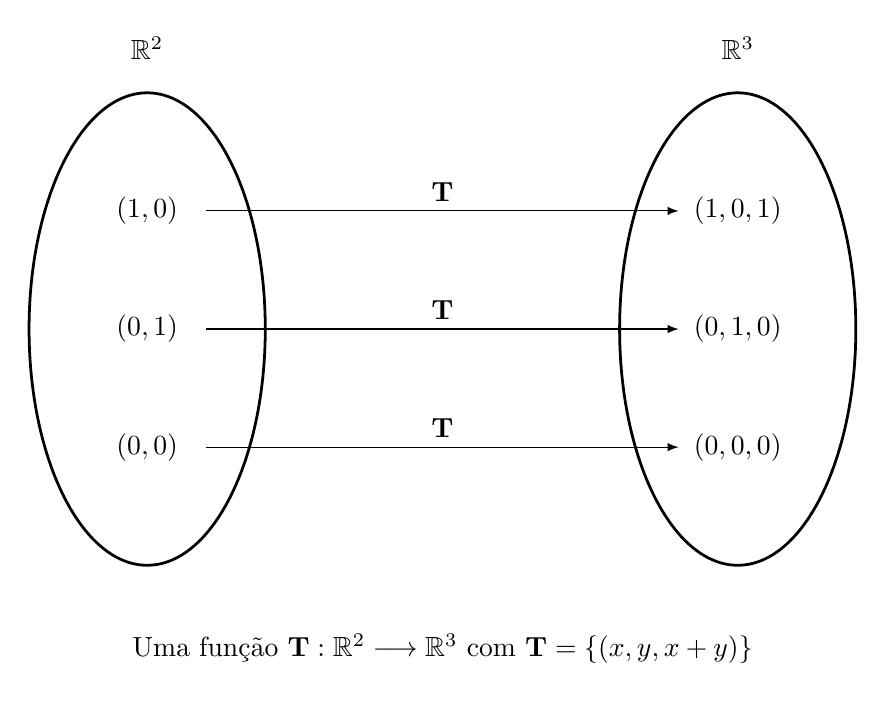
\begin{tikzpicture}[scale=1.5]
	\centering
	% Set A
	\draw[line width=1pt] (0,0) ellipse (1cm and 2cm);
	\node[above] at (0,2.2) (A) {$\mathbb{R}^2$};
	\node[centered] at (0,1) {$(1,0)$};
	\node[centered] at (0,0) {$(0,1)$};
	\node[centered] at (0,-1) {$(0,0)$};
	% Set B
	\draw[line width=1pt] (5,0) ellipse (1cm and 2cm);
	\node[above] at (5,2.2) (B) {$\mathbb{R}^3$};
	\node[centered] at (5,1) {$(1,0,1)$}; 
	\node[centered] at (5,0) {$(0,1,0)$};
	\node[centered] at (5,-1) {$(0,0,0)$};
	
	% Relations
	\draw[-latex, black] (0.5,1) -- node[midway, above] {$\mathbf{T}$} (4.5,1);
	\draw[-latex, black] (0.5, 0) -- node[midway, above] {$\mathbf{T}$} (4.5, 0);
	\draw[-latex, black] (0.5, -1) -- node[midway, above] {$\mathbf{T}$} (4.5, -1);
	
	% Label
	\node[below] at (2.5,-2.5) {Uma função $\mathbf{T}: \mathbb{R}^2 \longrightarrow \mathbb{R}^3$ com $\mathbf{T}=\{(x, y, x + y)\}$};
\end{tikzpicture}

\noindent\textbf{Exemplo 12:} Se tomarmos um vetor arbitrário e fazemos uma transformação linear idêntica, ou seja, $1\alpha$ = $\alpha$, é uma transformação linear de $\mathbf{V}$ em $\mathbf{V}$. A transformação é definida por $0\alpha = 0$, é também uma transformação linear de $\mathbf{V}$ em $\mathbf{V}$ \cite{hoffman1979}.

De acordo com o exemplo acima, percebe-se, que será uma função onde o gráfico passa a reta pela origem se supormos uma função afim, $\mathbb{R}^1$ em $\mathbb{R}^1$. Uma transformação linear mantém combinações lineares $W = [\mathbf{v}_1, \ldots, \mathbf{v}_n]$ são vetores que pertencem a $\mathbf{V}$ e possui seus escalares $c_1, \ldots, c_n$, então:

\centerline{$\mathbf{T}(c_1\mathbf{v}_1, \ldots, c_n\mathbf{v}_n) = \mathbf{T}(c_1\mathbf{v}_1 + c_2\mathbf{v}_2) = c_1(\mathbf{T}\mathbf{v}_1) + c_2(\mathbf{T}\mathbf{v}_2)$}


	
	\chapter{Aplicações de Transformações Lineares}
As TL têm contribuições significativas para o campo da AL. \cite{strang2010}, renomado matemático e professor do MIT - Massachusetts Institute of Technology, aborda, por exemplo, o processamento de sinais e imagens para compressão, filtragem, reconstrução e análise de dados, a análise de redes e sistemas dinâmicos da engenharia elétrica e ciência da computação, a geometria e a computação gráfica para manipular objetos em espaços tridimensionais, videogames e modelagem em três dimensões, além de cripto segurança e, mais recentemente, análise de dados em decisões gerenciais e aprendizagem de máquina. \nocite{pitombeira1971}

A seguir, baseando em um estudo desenvolvido na Universidade Federal de Alagoas \cite{sirlandro2017}, apresentamos algumas aplicações das TL na área de engenharia.

\section{Posicionamento de Um Braço Robótico}
Para executar atividades repetitivas, perigosas e precisas, um braço robótico, composto por elos e juntas conforme figura 12 é dispositivo dotado de articulações e pode ser programado utilizando aplicações de AL, considerando as variações de posição no plano e no espaço.

\begin{figure}[H]
	\centering
	\includegraphics[scale=1.00]{a_robo1.png}
	\caption{Esquema de articulações \cite{sirlandro2017}.}
\end{figure} 

Para representar a aplicação, considere que a figura 13a contém um braço robótico com dois graus de liberdade e seus comprimentos são indicados por $d_1, d_2 e d_3$ dos elos, e os ângulos da posição inicial do braço com base no ponto $\mathbf{P}$, nas coordenadas iniciais $(x_0, y_0)$. Na figura 13b, está demonstrada como seria o efeito desse movimento, com o ponto $\mathbf{P}$ na coordenada $(x_1, y_1)$, utilizando as TL.

\begin{figure}[H]
	\centering
	\includegraphics[scale=0.70]{a_robo2.png}
	\caption{Posição inicial e final \cite{sirlandro2017}.}
\end{figure} 

A Figura 14 apresenta o movimento de rotação e translação, e a figura 15 mostra o movimento de translação e rotação, observando que o resultado é diferente de acordo com a ordem aplicada.

\begin{figure}[H]
	\centering
	\includegraphics[scale=0.80]{a_robo3.png}
	\caption{Rotação e translação \cite{sirlandro2017}.}
\end{figure} 

\begin{figure}[H]
	\centering
	\includegraphics[scale=0.80]{a_robo4.png}
	\caption{Translação e rotação \cite{sirlandro2017}.}
\end{figure} 

Utilizando as TL, consideramos que o sistema adotado como global foi o do antebraço. Denominemos este sistema por $\{\mathbf{A}^0\}$. Onde $\mathbf{e}_1$ e $\mathbf{e}_2$ são os vetores da base canônica do $\mathbb{R}^2$, com origem no ponto $O$ (Figura 13b) e $d_1$ o comprimento do braço e de $\theta_1$ o ângulo que o antebraço faz com o eixo determinado por $\mathbf{e}_1$. Seja $\mathbf{A}_1 = \{f_1, f_2\}$ o sistema local obtido da rotação do sistema $\mathbf{A}_0$ pelo ângulo $\theta_1$ seguida da translação na direção de $\mathbf{e}_1$ por um comprimento $d_1$.

A partir da transformação de rotação, a matriz é representada por

\[
\mathbf{R}_1 = \begin{bmatrix}
	\cos\theta_1 & -\sin\theta_1 & 0\\
	 \sin\theta_1 & \cos\theta_1 & 0\\
	 0 & 0 & 1\\
\end{bmatrix}
\]

\noindent e sua respectiva matriz de translação na direção de $d_1\mathbf{e}_1$ é dada por

\[
\mathbf{T}_1 = \begin{bmatrix}
	1 & 0 & d_1\\
	0 & 1 & 0\\
	0 & 0 & 1\\
\end{bmatrix}
\]

Desta forma, a composição de $\mathbf{T}_1$ com $\mathbf{R}_1$ fica

\[
\mathbf{T}_1\cdot\mathbf{R}_1 = \begin{bmatrix}
	1 & 0 & d_1\\
	0 & 1 & 0\\
	0 & 0 & 1\\
\end{bmatrix}
\begin{bmatrix}
	\cos\theta_1 & -\sin\theta_1 & 0\\
	\sin\theta_1 & \cos\theta_1 & 0\\
	0 & 0 & 1\\
\end{bmatrix}
=
\begin{bmatrix}
	\cos\theta_1 & -\sin\theta_1 & d_1\\
	\sin\theta_1 & \cos\theta_1 & 0\\
	0 & 0 & 1\\
\end{bmatrix}
\]

Considerando que $d_2$ é o comprimento do antebraço e $\theta_2$ o ângulo que não faz com o eixo determinado for $f_1$, o sistema local $\mathbf{A}^2 = \{g_1, g_2\}$ é obtido da rotação do sistema $\mathbf{A}^1$ pelo ângulo $\theta_2$ seguida da translação, na direção de $f_1$, por um comprimento $d_2$, representado pela matriz de rotação

\[
\mathbf{R}_2 = \begin{bmatrix}
	\cos\theta_2 & -\sin\theta_2 & 0\\
	\sin\theta_2 & \cos\theta_2 & 0\\
	0 & 0 & 1\\
\end{bmatrix}
\]

\noindent e pela matriz de translação

\[
\mathbf{T}_2 = \begin{bmatrix}
	1 & 0 & d_2\\
	0 & 1 & 0\\
	0 & 0 & 1\\
\end{bmatrix}
\]

A composição $\mathbf{T}_2\cdot\mathbf{R}_2$ é representada por 

\[
\mathbf{T}_2\cdot\mathbf{R}_2 = \begin{bmatrix}
	1 & 0 & d_2\\
	0 & 1 & 0\\
	0 & 0 & 1\\
\end{bmatrix}
\begin{bmatrix}
	\cos\theta_2 & -\sin\theta_2 & 0\\
	\sin\theta_2 & \cos\theta_2 & 0\\
	0 & 0 & 1\\
\end{bmatrix}
=
\begin{bmatrix}
	\cos\theta_2 & -\sin\theta_2 & d_2\\
	\sin\theta_2 & \cos\theta_2 & 0\\
	0 & 0 & 1\\
\end{bmatrix}
\]

Então houve duas transformações sucessivas partindo do referencial global até o sistema local da mão. Agora partindo uma transformação que leva o referencial $\mathbf{A}^0$ ao referencial $\{\mathbf{A}^2\}$ como mostra a figura 16 abaixo.

\begin{figure}[H]
	\centering
	\includegraphics[scale=0.80]{a_robo5.png}
	\caption{Transformação do referencial $\mathbf{A}^0$ para o referencial $\{\mathbf{A}^2\}$ \cite{sirlandro2017}.}
\end{figure} 

Para levar $\mathbf{A}^0$ até $\mathbf{A}^2$ é necessário rotacionar (conforme demonstrado nos capítulos anteriores) e depois transladar, nessa ordem, por uma matriz do tipo

\[
\mathbf{T}\cdot\mathbf{R} = \begin{bmatrix}
	\cos\theta & -\sin\theta & d_1\\
	\sin\theta & \cos\theta & d_2\\
	0 & 0 & 1\\
\end{bmatrix}
\]

Nessa matriz, o ângulo $\theta$ que o referencial $\mathbf{A}^0$ deve ser rotacionado para ficar paralelo ao referencial $\mathbf{A}^2$ é $\theta_1 + \theta_2$. Além disso, note que as coordenadas do vetor translação $t = (t_1, t_2)$ para a transformação $\mathbf{T}\cdot\mathbf{R}$ são

\centerline{$t_1 = d_1 + d_2\cos\theta_1$}

\centerline{$t_2 = d_2\cos\theta_1$}

Então, a matriz de transformação do referencial $\mathbf{A}^0$ para o referencial $\mathbf{A}^2$ pode ser reescrita como 

\[
\mathbf{T}\cdot\mathbf{R} = \begin{bmatrix}
	\cos(\theta_1 + \theta_2) & -\sin(\theta_1 + \theta_2) & d_1 + d_2\cos\theta_1\\
	\sin(\theta_1 + \theta_2) & \cos(\theta_1 + \theta_2) & d_2\sin\theta_1\\
	0 & 0 & 1\\
\end{bmatrix}
\]

\noindent fazendo manipulações algébricas e reduzindo a matriz em um produto temos

\[
\mathbf{T}\cdot\mathbf{R} = \begin{bmatrix}
	\cos\theta_1 & -\sin\theta_1 & d_1\\
	\sin\theta_1 & \cos\theta_1 & 0\\
	0 & 0 & 1\\
\end{bmatrix}
\begin{bmatrix}
	\cos\theta_2 & -\sin\theta_2 & d_2\\
	\sin\theta_2 & \cos\theta_2 & 0\\
	0 & 0 & 1\\
\end{bmatrix}
=
\mathbb{T}_1\cdot\mathbf{R}_1 \bullet \mathbb{T}_2\cdot\mathbf{R}_2
\]

Observe a ordem que este produto deve ser realizado para obtermos a matriz final. Considere agora o referencial local $\mathbf{A}^3$, obtido ao transladarmos o referencial $\mathbf{A}^2$ para o ponto $P$ sem girá-lo. O ponto $P$ está localizado no sistema local $\mathbf{A}^2$ com coordenadas ($d_3, 0)$. É necessário, agora, apenas transladar de $\mathbf{A}^2$ para $P$ por meio da seguinte matriz (o ângulo de rotação é nulo)

\[
\mathbf{T}_3 = \begin{bmatrix}
	1 & 0 & d_3\\
	0 & 1 & 0\\
	0 & 0 & 1\\
\end{bmatrix}
\]

\noindent então, a matriz de transformação geral, M, é dada por 

\[
\mathbf{M} = \begin{bmatrix}
	\cos\theta_1 & -\sin\theta_1 & d_1\\
	\sin\theta_1 & \cos\theta_1 & 0\\
	0 & 0 & 1\\
\end{bmatrix}
\begin{bmatrix}
	\cos\theta_2 & -\sin\theta_2 & d_2\\
	\sin\theta_2 & \cos\theta_2 & 0\\
	0 & 0 & 1\\
\end{bmatrix}
\begin{bmatrix}
	1 & 0 & d_3\\
	0 & 1 & 0\\
	0 & 0 & 1\\
\end{bmatrix}
\]

Para encontrarmos as coordenadas do ponto $P$ no referencial $\mathbf{A}^0$ é necessário aplicar a matriz $\mathbf{M}$ ao vetor $(0, 0, 1)$, origem de $\mathbf{A}^0$. Então o ponto em análise pode ser expresso por

\centerline{$P = \mathbf{M}\cdot(0, 0, 1)$}

\noindent ou seja,

\[
P = \begin{bmatrix}
	\cos\theta_1 & -\sin\theta_1 & d_1\\
	\sin\theta_1 & \cos\theta_1 & 0\\
	0 & 0 & 1\\
\end{bmatrix}
\begin{bmatrix}
	\cos\theta_2 & -\sin\theta_2 & d_2\\
	\sin\theta_2 & \cos\theta_2 & 0\\
	0 & 0 & 1\\
\end{bmatrix}
\begin{bmatrix}
	1 & 0 & d_3\\
	0 & 1 & 0\\
	0 & 0 & 1\\
\end{bmatrix}
\begin{bmatrix}
	0\\
	0\\
	1\\
\end{bmatrix}
\]

\noindent realizando esse produto chegamos a 

\[
P = \begin{bmatrix}
	\cos(\theta_1 + \theta_2) & -\sin(\theta_1 + \theta_2) & d_1 + d_2\cos\theta_1 + cos(\theta_1 + \theta_2)d_3\\
	\sin(\theta_1 + \theta_2) & \cos(\theta_1 + \theta_2) & d_2\sin\theta_1 + \sin(\theta_1 + \theta_2)d_3\\
	0 & 0 & 1\\
\end{bmatrix}
\begin{bmatrix}
	0\\
	0\\
	1\\
\end{bmatrix}
\]

\noindent\textbf{Exemplo 15:} Seja a posição inicial do braço robótico dada pela figura 17, onde $d_1 = 20cm, d_2 = 30cm, d_3 = 14cm, \theta_1 = 60^{\circ}$ e $\theta_2 = -90^{\circ}$.

\noindent\textbf{a)} Determinar as coordenadas do ponto $P$ para esta configuração em relação ao sistema global e \textbf{b)} para $\theta_1 = 45^{\circ}$ e $\theta_2 = 45^{\circ}$.

\begin{figure}[H]
	\centering
	\includegraphics[scale=1.00]{a_robo6.png}
	\caption{Posição inicial do braço robótico $\{\mathbf{A}^2\}$ \cite{sirlandro2017}.}
\end{figure} 

\noindent\textbf{a)} O ponto $P$ é obtido diretamente pela inserção direta dos valores fornecidos

\[
P = \begin{bmatrix}
	\cos(-30) & -\sin(-30) & 20 + 30\cos(60)+ cos(-30)14\\
	\sin(-30) & \cos(-30) & 30\sin(60) + \sin(-30)14\\
	0 & 0 & 1\\
\end{bmatrix}
\begin{bmatrix}
	0\\
	0\\
	1\\
\end{bmatrix}
\]

\[
P = \begin{bmatrix}
	47,12\\
	19\\
	1\\
\end{bmatrix}
\]

\noindent\textbf{b)} O ponto $P$ é obtido diretamente pela inserção direta dos valores fornecidos

\[
P = \begin{bmatrix}
	\cos(90) & -\sin(90) & 20 + 30\cos(45)+ cos(90)14\\
	\sin(90) & \cos(90) & 30\sin(45) + \sin(90)14\\
	0 & 0 & 1\\
\end{bmatrix}
\begin{bmatrix}
	0\\
	0\\
	1\\
\end{bmatrix}
\]

\[
P = \begin{bmatrix}
	41,2\\
	3,2\\
	1\\
\end{bmatrix}
\]

\section{Aplicação das Transformações Lineares na Educação}
É previsto na Base Nacional Comum Curricular \cite{brasil_bncc2018} que estudantes do Ensino Médio adquiram as competências de:

\begin{itemize}
	\item Utilizar estratégias, conceitos e procedimentos matemáticos para interpretar situações em diversos contextos, sejam atividades cotidianas, sejam fatos das Ciências da Natureza e Humanas, das questões socioeconômicas ou tecnológicas, divulgados por diferentes meios, de modo a contribuir para uma formação geral. 
	\item Propor ou participar de ações para investigar desafios do mundo contemporâneo e tomar decisões éticas e socialmente responsáveis, com base na análise de problemas sociais, como os voltados a situações de saúde, sustentabilidade, das implicações da tecnologia no mundo do trabalho, entre outros, mobilizando e articulando conceitos, procedimentos e linguagens próprios da Matemática. 
	\item Utilizar estratégias, conceitos, definições e procedimentos matemáticos para interpretar, construir modelos e resolver problemas em diversos contextos, analisando a plausibilidade dos resultados e a adequação das soluções propostas, de modo a construir argumentação consistente. 
	\item Compreender e utilizar, com flexibilidade e precisão, diferentes registros de representação matemáticos (algébrico, geométrico, estatístico, computacional etc.), na busca de solução e comunicação de resultados de problemas. 
	\item Investigar e estabelecer conjecturas a respeito de diferentes conceitos e propriedades matemáticas, empregando estratégias e recursos, como observação de padrões, experimentações e diferentes tecnologias, identificando a necessidade, ou não, de uma demonstração cada vez mais formal na validação das referidas conjecturas.
\end{itemize}

Em específico, a habilidade (EM13MAT301), que requer que a pessoa estudante possa resolver e elaborar problemas do cotidiano, da Matemática e de outras áreas do conhecimento, que envolvem equações lineares simultâneas, usando técnicas algébricas e gráficas, com ou sem apoio de tecnologias digitais.

A partir das bases de AL formadas no Ensino Médio, é esperado que estudantes da área de exatas desenvolvam pensamento matemático de forma avançada em cursos de Engenharia, Física Aplicada, entre outros. Para que o ensino aprendizagem seja sólido, professores devem oportunizar a reflexão dos objetos da disciplina além de definir e exemplificar os conceitos. \cite{marins_savioli_2016}, não sendo apenas uma questão específica brasileira, e sim mundial \cite{pena2016}.

Com o auxílio do software GeoGebra, é possível experimentar dinâmicas e visualizações da TL \cite{eliza2015}, facilitando a compreensão e aplicação dos conceitos apresentados de forma mais dinâmica e efetiva na construção do conhecimento \cite{souzasilzaeliza2017}.

\section{Aplicação em Criptografia}
A criptografia, modelo de segurança cibernética, nada mais é que um método de armazenar e transmitir dados de um forma que somente às pessoas autorizadas como, por exemplo, os destinatários, possam ler e processar \cite{helio2009}. Então, é um método extremamente eficaz para proteção de ataques cibernéticos em busca de informações sensíveis, dados de clientes, contas bancárias e entre outros.

Com advento e vigência em 2020 a LGPD (Lei Geral de Proteção de Dados Pessoais), se tornou cada vez mais intrínseco o uso de modelos de segurança para a proteção de dados, uma codificação forte para resolver brechas de segurança. Porém, há duas condições para importantes na criptografia de dados:

\begin{enumerate}
	\item Não existe um método de criptografia que não possa ser quebrado.
	\item O real objetivo da criptografia é fazer com que conseguir acesso à informação, seja tão trabalhoso e leve ao mesmo tempo, que o atacante sinta-se desestimulado e desista.
\end{enumerate}

Usando um operador linear no $\mathbb{R}^2$, imaginemos que a mensagem a seguir tenha grande valor de especulação, e que seu remetente e seu destinatário sejam conhecidos:

\centerline{O texto puro é: C-O-N-V-E-N-I-O-U-N-I-V-I-M-A-U-F-S-C-M-T-M}

\begin{table}[h]
	\centering
	\begin{tabular}{@{} *{13}{c} @{}}
		\toprule
		\textbf{A} & \textbf{B} & \textbf{C} & \textbf{D} & \textbf{E} & \textbf{F} & \textbf{G} & \textbf{H} & \textbf{I} & \textbf{J} & \textbf{K} & \textbf{L} & \textbf{M} \\
		\midrule
		6 & 14 & -2 & 7 & -8 & -6 & 13 & -7 & 2 & -4 & -3 & 3 & 10 \\
		\toprule
		\textbf{N} & \textbf{O} & \textbf{P} & \textbf{Q} & \textbf{R} & \textbf{S} & \textbf{T} & \textbf{U} & \textbf{V} & \textbf{W} & \textbf{X} & \textbf{Y} & \textbf{Z} \\
		\midrule
		15 & 1 & -9 & 8 & -5 & 11 & 0 & 4 & 9 & -1 & 12 & 21 & 5 \\
		\bottomrule
	\end{tabular}
	\caption{Tabela de randomização \cite{helio2009}}
\end{table}

A tabela acima é o que chamamos de randomizar, cada letra está relacionada com um número na linha logo abaixo.

Vamos fazer a primeira cifragem:

\begin{verbatim}
	-2_1_15_9_-8_15_2_1_4_15_2_9_2_10_6_4_-6_11_-2_10_0_10
\end{verbatim}

O algoritmo que usaremos é o Operador Linear do $\mathbb{R}^2$

\centerline{$T(x, y) = (3x -y, 2x + y)$}

Primeiramente, vamos confirmar que $T$ é um Isomorfismo, através de sua matriz associada na base canônica do $\mathbb{R}^2$, é inversível, ou seja, se seu determinante é diferente de zero:

\centerline{$[T] = \begin{pmatrix} 3 & -1 \\ 2 & 1 \end{pmatrix}$ e $\det[T] = 3 -(-2) = 5$},

\noindent realmente, $[T]$ é inversível, logo, $T$ é um Isomorfismo. Tomando de dois em dois números, e fazendo as contas:

\begin{center}
	T(-2, 1) = (3(-2) -1, 2(-2) + 1) = (-7, -3)
	
	T(15, 9) = (3(15) – 9, 2(15) + 9) = (36, 39)
	
	T(-8, 15) = (3(-8) – 15, 2(-8) + 15) = (-39, -1)
		
	T(2, 1)  = (3(2) – 1, 2(2) + 1) = (5, 5)
	
	T(4, 15)  = (3(4) – 15, 2(4) + 15) = (-3, 23)
	
	T(2, 9) = (3(2) – 9, 2(2) + 9) = (-3, 13)
	
	T(2, 10) = (3(2) – 10, 2(2) + 10) = (-4, 14)
	
	T(6, 4) = (3(6) – 4, 2(6) + 4) = (14, 16)
	
	T(-6, 11) = (3(-6) – 11, 2(-6) + 11) = (-29, -1)
	
	T(-2, 10) = (3(-2) – 10, 2(-2) + 10) = (-16, 6)
	
	T(0, 10) = (3(0) – 10, 2(0) + 10) = (-10, 10)
\end{center}

Aqui fazemos a segunda cifragem:

\begin{verbatim}
	-7_-3_36_39_-39_-1_5_5_-3_23_-3_13_-4_14_14_16_-29_-1_-16_6_-10_10
\end{verbatim}

Este é o texto recebido pelo destinatário. Cabe ao destinatário decifrar, o texto recebido.

São de domínio comum ao remetente e do destinatário, a tabela de
randomização que faz parte do algoritmo criptográfico. Neste caso $T(x, y) = (3x -y, 2x + y)$ assim o destinatário deverá encontrar
o Isomorfismo Inverso de $T$, aqui usaremos o processo prático via escalonamento de matrizes, para obtermos a inversa de $[T]$ e assim chegarmos a $T^{-1}$:

$
\begin{pmatrix}
	 3 & -1 & 1 & 0 \\
	 2 & 1 & 0 & 1 \\ 
	 \end{pmatrix}
	 \sim 1/3 L_1 \rightarrow L_1 \sim
\begin{bmatrix}
	1 & 1/3 & 1/3 & 0 \\
	2 & 1 & 0 & 1 \\
\end{bmatrix}
	\sim 1/2 L_2 \rightarrow L_2 \sim
$

$
\begin{pmatrix}
	1 & -1/3 & 1/3 & 0 \\
	1 & 1/2 & 0 & 1/2 \\
\end{pmatrix}
	\sim L_2 - L_1 \rightarrow \sim
\begin{pmatrix}
	1 & -1/3 & 1/3 & 0 \\
	0 & 5/6 & -1/3 & 1/2 \\
\end{pmatrix}
	\sim 6/5 L_2 \rightarrow L_2 \sim
$

$
\begin{pmatrix}
	1 & -1/3 & 1/3 & 0 \\
	0 & 1 & -2/5 & 3/5 \\
\end{pmatrix}
\sim L_1 + 1/3 L_2 \sim
\begin{pmatrix}
	1 & 0 & 1/5 & 1/5 \\
	0 & 1 & -2/5 & 3/5 \\
\end{pmatrix}
$

\noindent então, 
$[T^{-1}] = 1/5
\begin{pmatrix}
	1 & 1 \\
	-2 & 3 \\
\end{pmatrix}
$ e assim, $1/5
\begin{pmatrix}
	1 & 1 \\
	-2 & 3 \\
\end{pmatrix}
	\cdot
\begin{pmatrix}
	x \\ y
\end{pmatrix}
= 1/5\begin{pmatrix}
	x + y \\
	3y -2x
\end{pmatrix}
$

Logo, $T^{-1}(x, y) = (1/5(x + y), 1/5(3y -2x))$

\centerline{$T^{-1}$(-7, -3) = (1/5(-7-3), 1/5(3[-3] – 2[-7])) = (-2, 1)}

\centerline{$T^{-1}$(36, 39) = (1/5(36+39), 1/5(3[39] – 2[36])) = (15, 9)}

\centerline{$T^{-1}$(-39, -1) = ((1/5(-39-1), 1/5(3[-1] – 2[-39])) = (-8, 15)}

\centerline{$T^{-1}$(5, 5) = (1/5(5 + 5), 1/5(3[5] – 2[5])) = (2, 1)}

\centerline{$T^{-1}$(-3, 23) = (1/5(-3+23), 1/5(3[23] – 2[-3])) = (4, 15)}

\centerline{$T^{-1}$(-3, 13) = (1/5(-3+13), 1/5(3[13] – 2[-3])) = (2, 9)}

\centerline{$T^{-1}($-4, 14) = (1/5(-4+14), 1/5(3[14] – 2[-4])) = (2, 10)}

\centerline{$T^{-1}$(14, 16) = (1/5(14+16), 1/5(3[16] – 2[14])) = (6, 4)}

\centerline{$T^{-1}$(-29, -1) = ((1/5(-29-1), 1/5(3[-1] – 2[-29])) = (-6, 11)}

\centerline{$T^{-1}$(-16, 6) = (1/5(-16+6), 1/5(3[6] – 2[-16])) = (-2, 10)}

\centerline{$T^{-1}$(-10, 10) = (1/5(-10+10), 1/5(3[10] – 2[-10])) = (0, 10)}

Novamente, aplicando a tabela de randomização:

\begin{table}[h]
	\centering
	\begin{tabular}{@{} *{13}{c} @{}}
		\toprule
		\textbf{A} & \textbf{B} & \textbf{C} & \textbf{D} & \textbf{E} & \textbf{F} & \textbf{G} & \textbf{H} & \textbf{I} & \textbf{J} & \textbf{K} & \textbf{L} & \textbf{M} \\
		\midrule
		6 & 14 & -2 & 7 & -8 & -6 & 13 & -7 & 2 & -4 & -3 & 3 & 10 \\
		\toprule
		\textbf{N} & \textbf{O} & \textbf{P} & \textbf{Q} & \textbf{R} & \textbf{S} & \textbf{T} & \textbf{U} & \textbf{V} & \textbf{W} & \textbf{X} & \textbf{Y} & \textbf{Z} \\
		\midrule
		15 & 1 & -9 & 8 & -5 & 11 & 0 & 4 & 9 & -1 & 12 & 21 & 5 \\
		\bottomrule
	\end{tabular}
	\caption{Tabela de randomização \cite{helio2009}}
\end{table}

\noindent e finalmente, o texto descriptografado:

\centerline{CONVENIO UNIVIMA UFSC MTM}

A transformação linear aplicada, usada como algoritmo, mistura de duas em duas letras a palavra.

\section{Classificação de Imagens com Redes Neurais}

Considere uma rede neural artificial que é treinada para classificar imagens em categorias diferentes, como gatos e cachorros. A rede neural tem uma camada de entrada que recebe as características das imagens, uma camada oculta que processa essas características e uma camada de saída que produz a classificação final.

A camada oculta é composta por neurônios que realizam transformações lineares seguidas de funções de ativação não-lineares. Por exemplo, um neurônio pode ser representado pela seguinte equação:

\begin{equation}
	h = Wx + b
\end{equation}

onde $W$ é a matriz de pesos, $x$ é o vetor de entrada e $b$ é o vetor de bias. Essa equação representa a combinação linear dos pesos $W$ com a entrada $x$ e o bias $b$.

Para demonstrar que essa transformação é linear, podemos aplicar a lei de composição de funções matemáticas:

\begin{equation}
	h = Wx + b = W(x + 0) + b = Wx + W(0) + b = Wx + b
\end{equation}

Essa equação demonstra que a transformação é linear, pois a combinação de $W$ com $x$ e $b$ não altera a estrutura linear da equação.

A aplicação de uma função de ativação não-linear sobre $h$ introduz a não-linearidade necessária para a aprendizagem de padrões complexos. Por exemplo, a função de ativação sigmoide pode ser representada pela seguinte equação:

\begin{equation}
	\sigma(h) = \frac{1}{1 + e^{-h}}
\end{equation}

Essa função de ativação não-linear permite que a rede neural aprenda a classificar imagens complexas, como imagens de gatos e cachorros.

De acordo com \cite{lecun2015}, a utilização de transformações lineares em redes neurais tem se mostrado eficaz na resolução de problemas de classificação e regressão em inteligência artificial.

	
	% Conclusão
	\chapter{Conclusão}
That's all folks!
Teste citação: De acordo com \cite{einstein1905}, a teoria da relatividade restrita foi publicada por Einstein em 1905.

		
	% Referências Bibliográficas
	\bibliographystyle{abntex2-alf}
	\bibliography{references.bib}

		
\end{document}